\chapter{软件需求规格说明书}

\section{功能需求}

\subsection{管理人员需求}
\begin{itemize}
    \item{商家使用}:商家能够注册并向平台提供自己的店铺信息,注册店铺。!!
    \item{用户使用}:用户可以注册登录,进行下单。!!
    \item{店铺排行}:根据打分,销量进行综合排名餐馆。!
    \item{餐食排行}:给菜品显示销量,并且在店家可以自主推主打菜的同时,单独显示一个分区为食客推荐或根据销量之类的。!
    
    \item{大数据推送}:看人上菜,为食客献上他可能喜欢的店。*
    \item{费用抽成}:平台在每单交易中进行抽成。*
    
    \item{骑手指派}:根据骑手的位置,评价是否合格进行推送订单,且在一名骑手接受后,撤销其他推送,允许骑手短时间内取消配送并重新指派。?
    \item{外卖员使用}:外卖员可以注册登录并且通过平台接单。?(外卖员部分需要和定位有关,不知道需不需要)
\end{itemize}


\subsection{用户需求}
\subsubsection{普通用户需求}
\begin{itemize}
    \item{下单流畅}:使用时应该流畅,能够随时中断,随时返回到上一页面以及返回主页等页面。并且在订单未支付时候返回,应该保留历史订单,之后支付。!!
    \item{购物透明}:能够随时看到自己已经购入了什么,需要花费多少;正确显示历史购买记录。!!
    \item{方便日常}:可以将喜欢的商家添加至收藏夹。可以保存多个地址在下单时候进行选择。!!
    \item{给予反馈}:可以为商家、骑手打评分,以及向平台对商家进行举报。!
    
    \item {个性化}:主题,字体大小颜色可供选择。*
    \item {取消订单}:在一定时间内可以取消订单。*
    \item{预估时间}:可以看到订餐后预计送达时间。*(涉及定位)
    
    \item {派送透明}:可以向商家、骑手查询自己外卖的进度。?
    \item{tobecontinue}……
\end{itemize}

\subsubsection{商家用户需求}
\begin{itemize}
    \item {营业时间}:非营业时间不接受订单。!
    \item {差评申诉}:对于不合理的差评,可以向平台申诉申请取消。!
    \item {上架商品}:可以上架商品,并且推出主打菜。!!
    
    \item{平台推送}:通过与平台沟通交易,向平台商议(购买)推送。*
    \item {店铺优惠}:自己店铺搞活动发送优惠卷等物品,向平台申请,由平台发放给用户。*
\end{itemize}

\subsubsection{骑手需求?}
\begin{itemize}
    \item {差评申诉}:对于不合理的差评,可以向平台申诉申请取消。?
    \item {取消订单}:骑手在误触接受订单后,短时间内可以无条件取消;已经有突发事故,可以通过扣除信誉分的方式取消。?
\end{itemize}


\section{非功能需求}
可以在各种机型中正确显示页面。用户的隐私和数据应该封闭且安全。!!

\section{UML图}
注册与登录如图
\begin{figure}[htbp]
    \centering
    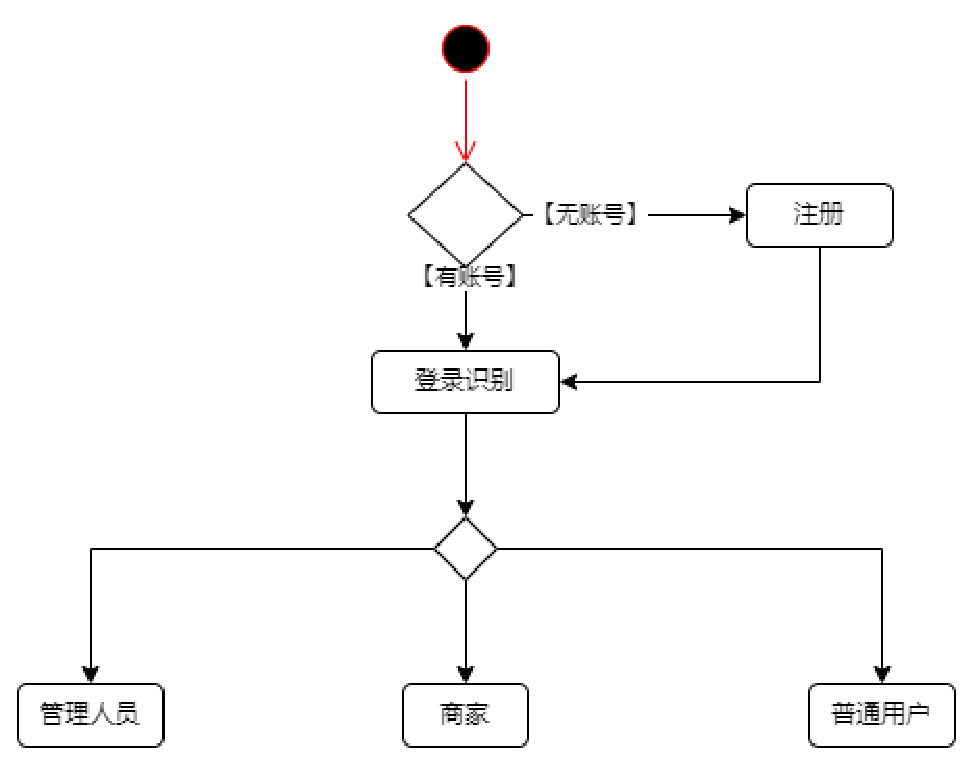
\includegraphics[width=1\textwidth]{login}
    \caption{注册与登录活动图}\label{fig:ds}
\end{figure}

用户如何成为商家如图\ref{fig:dd}
\begin{figure}[htbp]
    \centering
    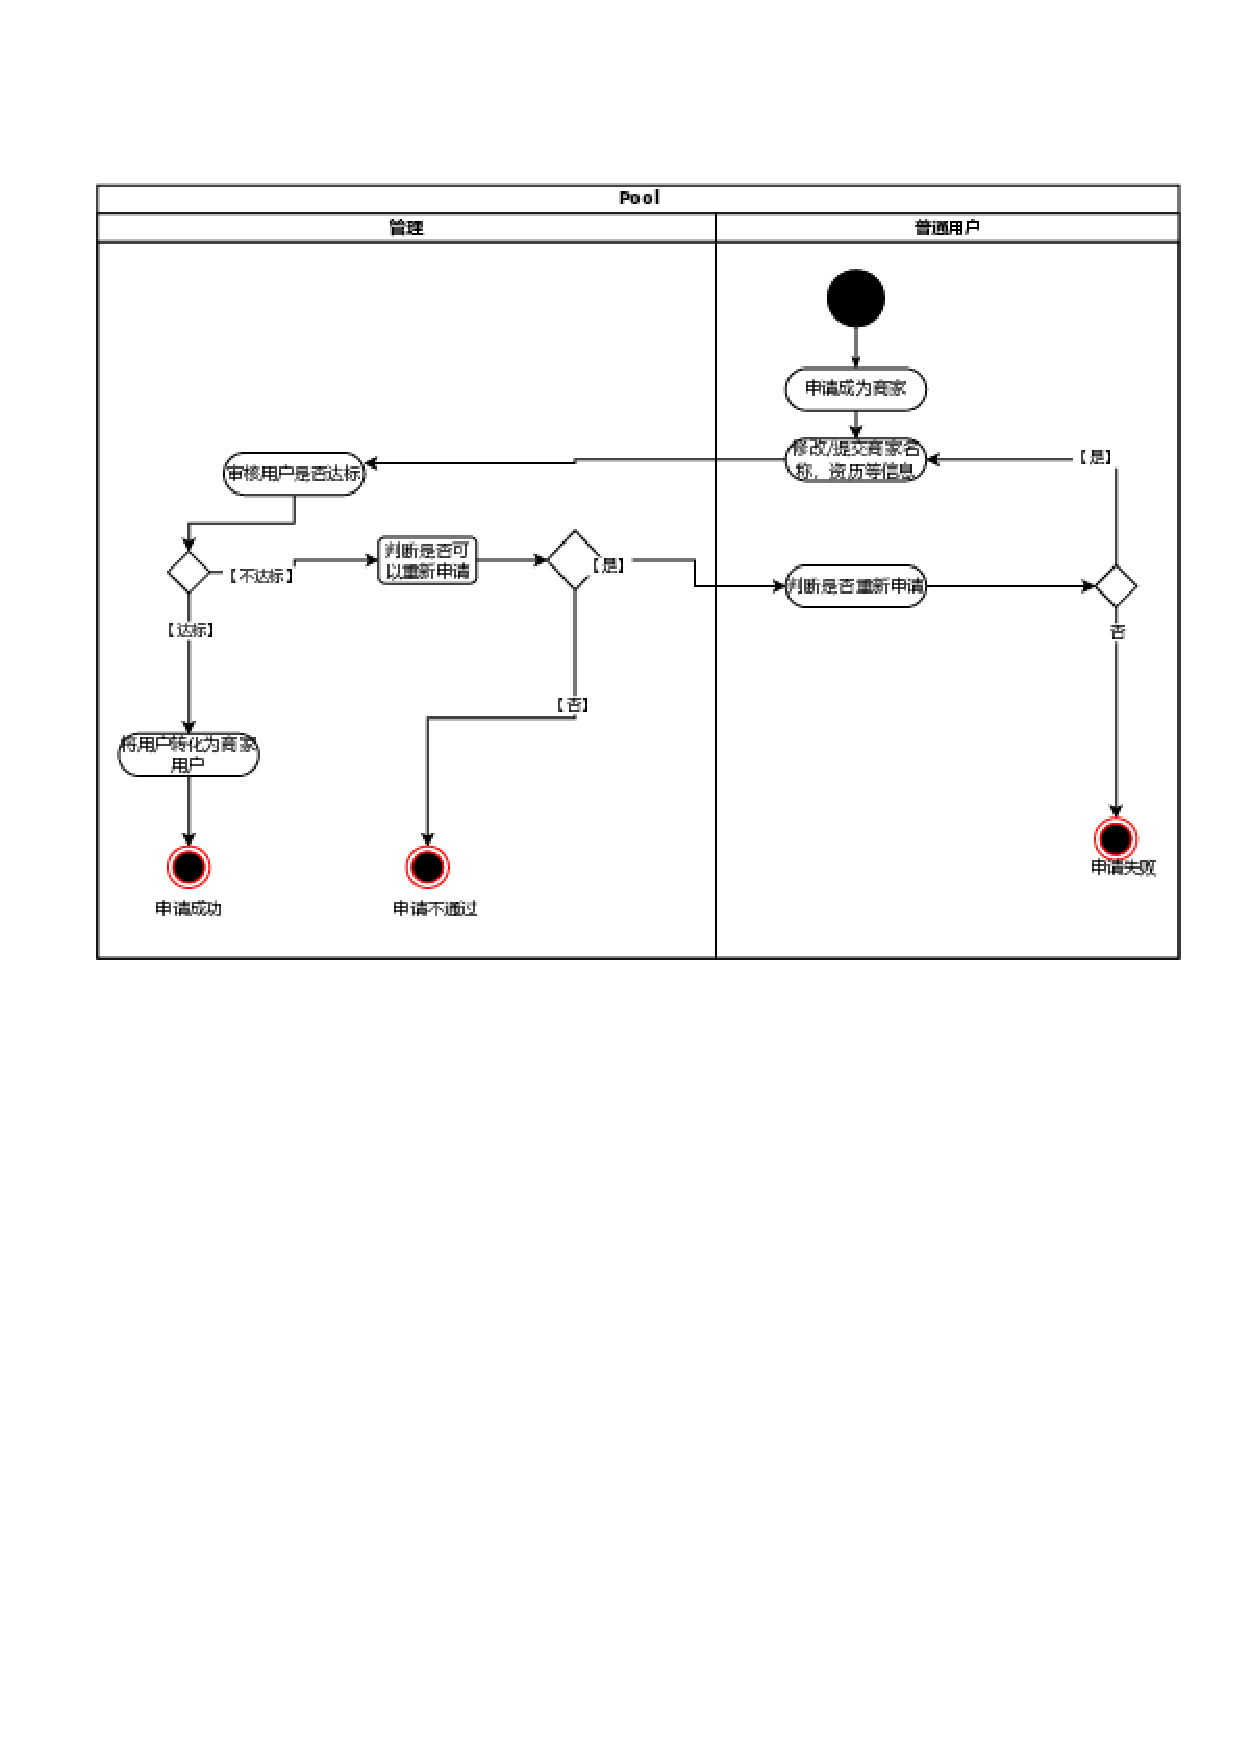
\includegraphics[width=1\textwidth]{utobe}
    \caption{用户转化为商家}\label{fig:dd}
\end{figure}
